\section{Uvod}

Ovaj rad se bavi modeliranjem dela sistema Nacionalne slu\v zbe za zapo\v sljavanje republike Srbije. U okviru ovog rada, obra\' cena je pa\v znja i na mogu\' ca unapre\dj enja sistema.\\

Rad je izra\dj en kao timski studentski projekat na Matemati\v ckom fakultetu, na studijskom programu Informatika, prve godine Master studija. Projekat je odra\dj en pod nadzorom profesora dr Sa\v se Malkova, u okviru predmeta Informacioni sistemi.\\

U nastavku \' cemo detaljnije opisati rad Nacionalne slu\v zbe.

\subsection{Nacionalna slu\v zba za zapo\v sljavanje}

Nacionalna slu\v zba za zapo\v sljavanje (u daljem tekstu Nacionalna slu\v zba) obavlja poslove zapo\v sljavanja, osiguranja za slu\v caj nezaposlenosti, ostvarivanje prava iz osiguranja za slu\v caj nezaposlenosti i druga prava u skladu sa zakonom, odnosno poslove vo\dj enja evidencija u oblasti zapo\v sljavanja, kao i stru\v cno-organi\-zacione, upravne, ekonomsko-finansijske i druge op\v ste poslove u oblasti zapo\v sljavanja i osiguranja za slu\v caj nezaposlenosti, u skladu sa zakonom, svojim statutom i drugim aktima Nacionalne slu\v zbe.

\begin{mylandscape}
	\subsubsection{Dijagram konteksta}
	
	\begin{figure}[H]
		\centering
		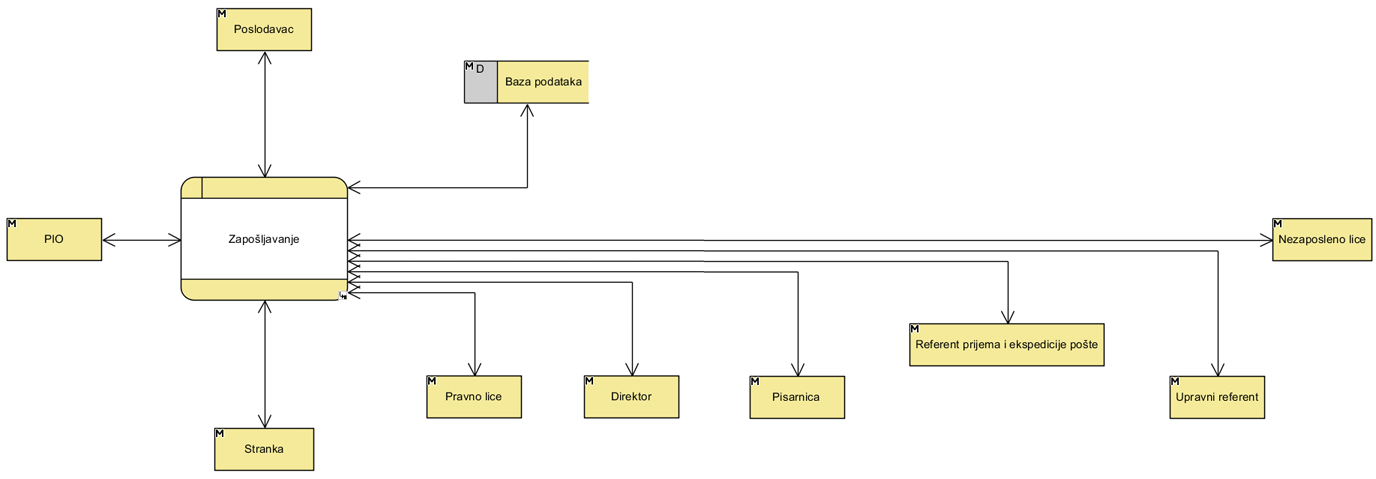
\includegraphics[width=0.8\paperwidth]{dijagrami/dijagrami-toka-podataka/zaposljavanje-dijagram-konteksta.png}
		\caption{Dijagram konteksta — prikaz sistema kao proces ''Zapo\v sljavanje''.}
		\label{dtp: dijagram konteksta}
	\end{figure}

	\newpage
	
	\begin{figure}[H]
		\centering
		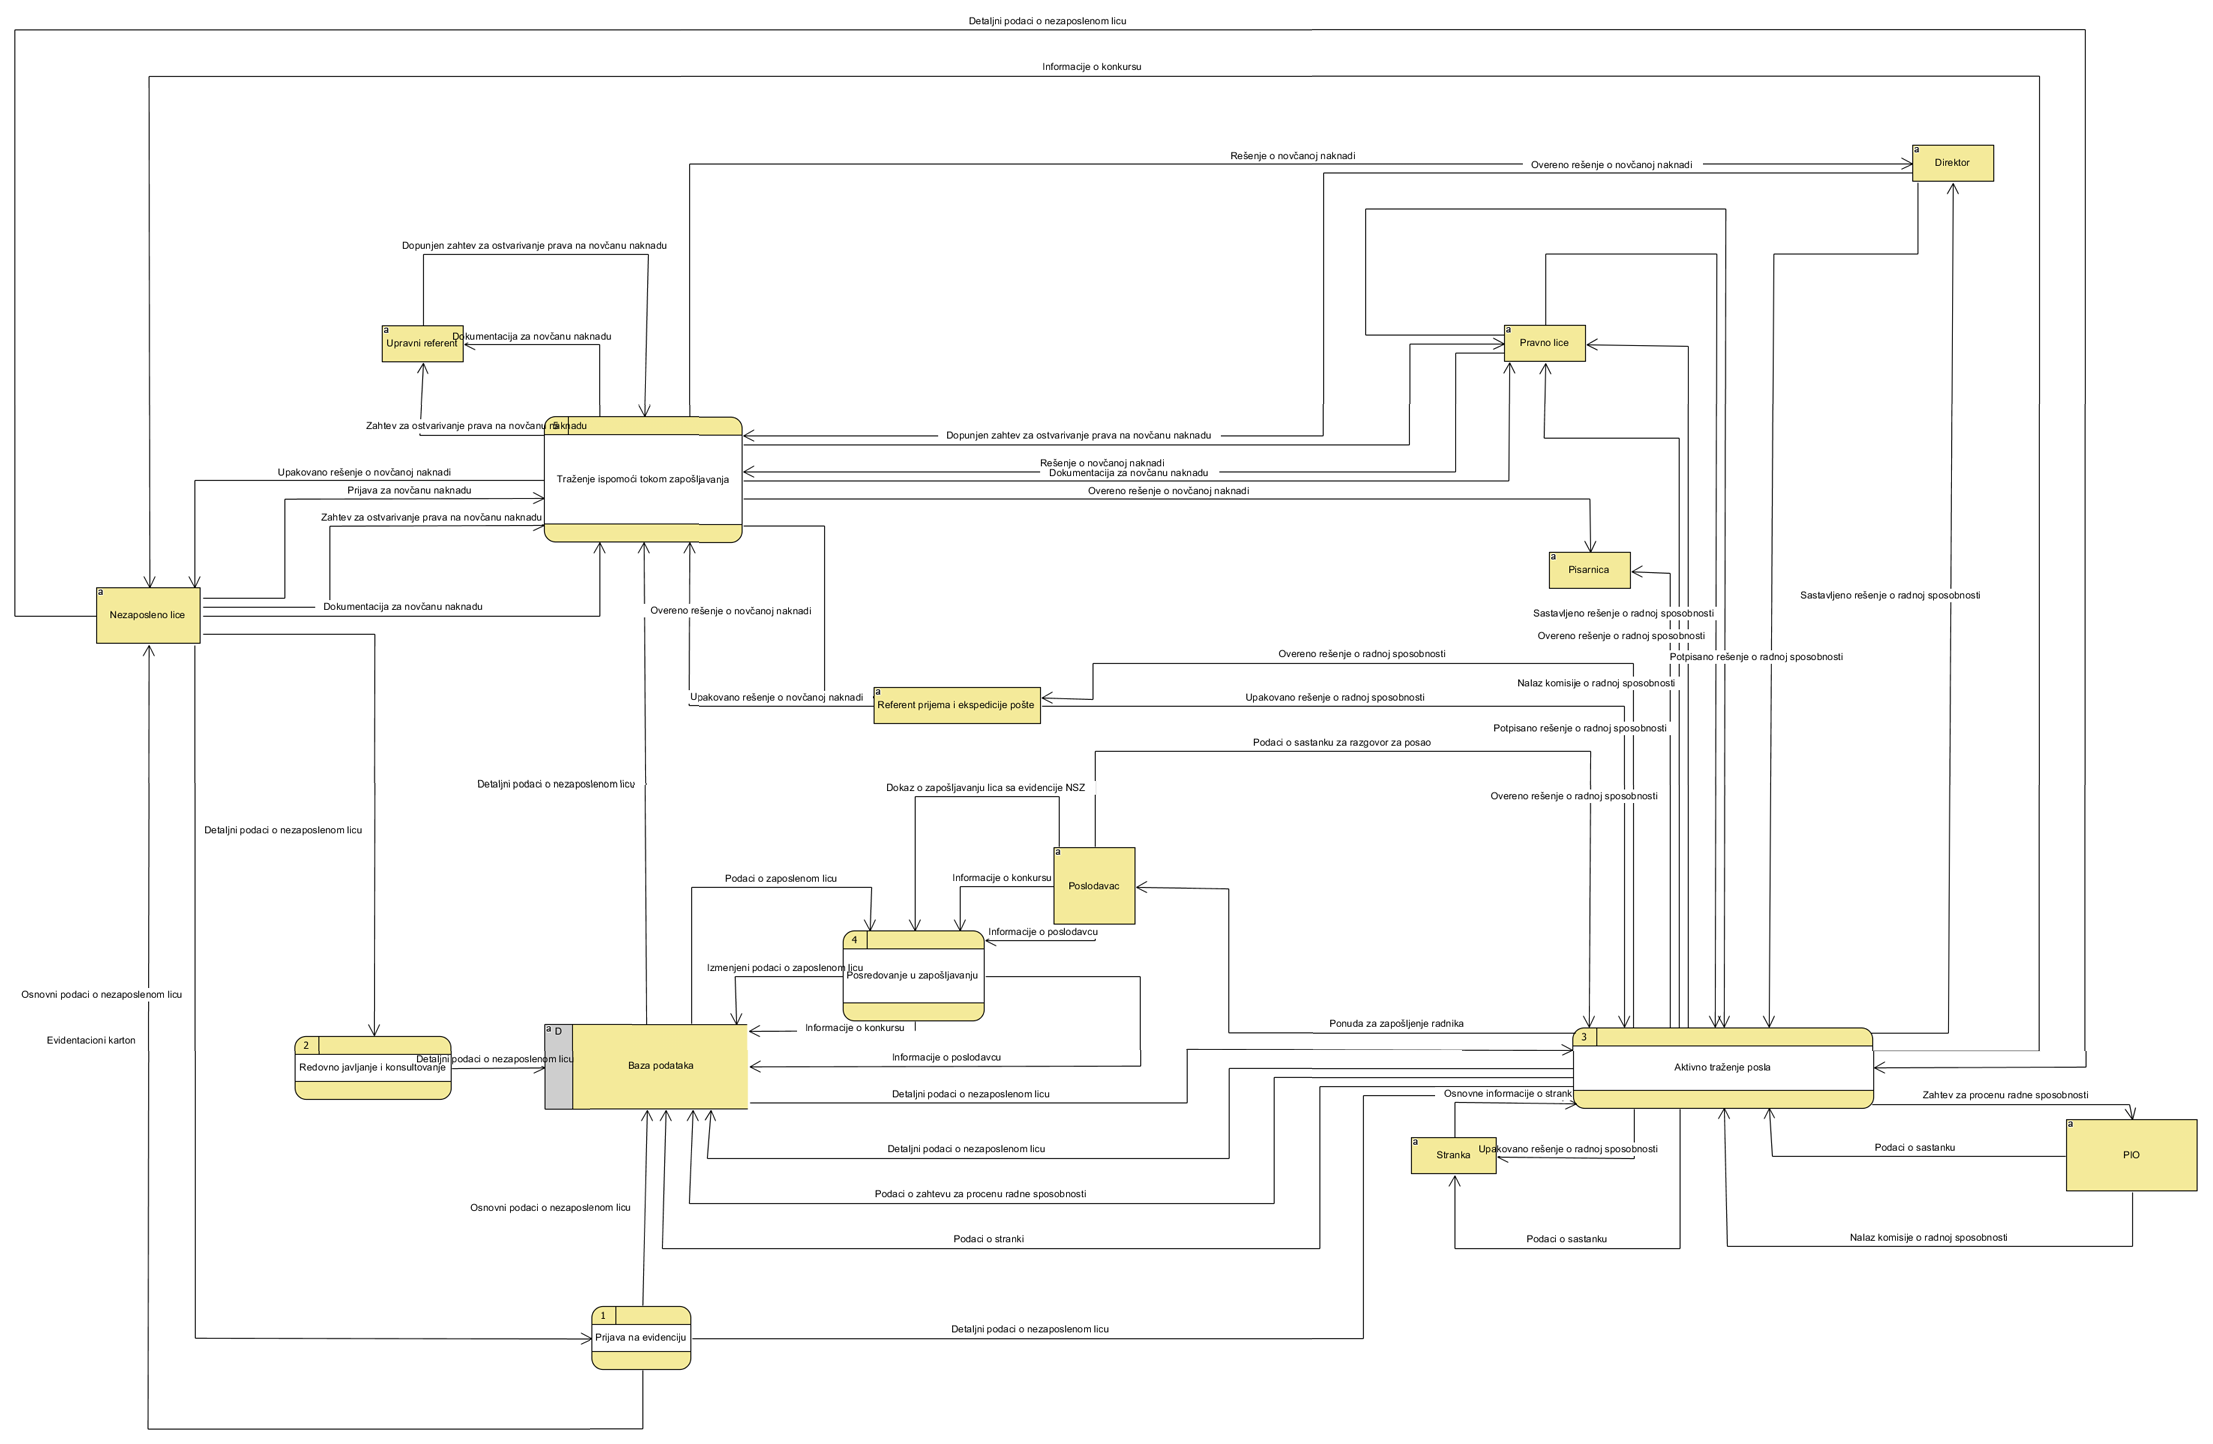
\includegraphics[width=0.7\paperwidth]{dijagrami/dijagrami-toka-podataka/zaposljavanje-dtp-nivoa-0.png}
		\caption{Dekompozicija procesa ''Zapo\v sljavanje'' (Slika \ref{dtp: dijagram konteksta}).}
	\end{figure}

\end{mylandscape}

\subsection{Metodologija rada}

Prilikom izrade rada, informacije o Nacionalnoj slu\v zbi su prikupljene iz dva glavna izvora. Prvi izvor predstavljaju zvani\v cna dokumenta Nacionalne slu\v zbe, i to ''Program rada Nacionalne slu\v zbe za zapo\v sljavanje (za 2016. godinu)'' i ''Statut Nacionalne slu\v zbe za zapo\v sljavanje'', \v cijim razmatranjem smo dolazili do formalnih informacija o sistemu. Drugi izvor informacija je razgovor sa zaposlenim licima, \v sto nam je prevashodno omogu\' cilo da steknemo uvid u mogu\' ca unapre\dj enja sistema.\\

Deo sistema koji je analiziran je modeliran kori\v s\' cenjem razli\v citih dijagramskih tehnika. U daljem tekstu \'cemo navesti kori\v s\'cene tehnike i dati ukratke opise.\\

Zahtevi sistema su modelirani dijagramima slu\v cajeva upotrebe (engl. \textit{Use Case Diagram}). Slu\v caj upotrebe je niz koraka pona\v sanja (scenario), automatskih i ru\v cnih, koji slu\v ze za kompletiranje jednog poslovnog zadatka. Dijagram slu\v cajeva upotrebe prikazuje interakciju izme\dj u sistema i eksternih sistema i korisnika. Drugim re\v cima, on grafi\v cki predstavlja ko \' ce koristiti sistem i na koje na\v cine korisnik mo\v ze da interaguje sa sistemom (\cite{SADM}). Dijagrami slu\v cajeva upotrebe su dopunjeni BPMN dijagramima i dijagramima sekvence.\\

\textit{Business Process Model and Notation} (skra\' ceno, BPMN) standard je za modeliranje poslovnih procesa koji obezbe\dj uje grafi\v cku notaciju za preciziranje poslovnih procesa. Cilj BPMN je da podr\v zi modeliranje poslovnih procesa za tehni\v cke i netehni\v cke (poslovne) korisnike nude\' ci notaciju koja je intuitivna poslovnim licima, a opet dovoljno jaka da mo\v ze da predstavi kompleksnu procesnu semantiku (\cite{BPMN}). Dakle, BPMN dijagrame (posebno, BPMN dijagrame saradnji) koristi\' cemo za opisivanje interakcije izme\dj u entiteta tokom slu\v cajeva upotrebe.\\

Dijagrami sekvence (engl. \textit{Sequence Diagram}) ilustruju objekte koji u\v cestvuju u slu\v caju upotrebe i poruke koje se razmenjuju izme\dj u njih u toku vremena, u jednom slu\v caju upotrebe (\cite{SAAD}). Ove dijagrame \' cemo koristiti pri slu\v cajevima upotrebe za koje smatramo da je potrebno dodatno opisati tok scenarija u vremenu.\\

Dijagram stanja (engl. \textit{state diagram} ili \textit{state machine diagram}) predstavlja dinami\v cki model koji prikazuje razli\v cita stanja kroz koje jedna klasa prolazi tokom svog \v zivota (\cite{SAAD}).\\

Dijagrami toka podataka (engl. \textit{Data Flow Diagrams}) predstavljaju jednu od osnovnih tehnika strukturnih metodologija. DTP opisuju na koji na\v cin se kre\' cu podaci kroz sistem. Razlikujemo nivoe DTP, pa tako dijagram konteksta predstavlja DTP najvi\v seg nivoa i njime se \v citav sistem (podsistem) predstavlja kao jedan proces (\cite{smalkov-slajdovi}). Dijagram konteksta \' cemo koristiti upravo da bismo pokazali granice sistema i komunikaciju sa njegovim okru\v zenjem.\\

Dijagram klasa (engl. \textit{Class Diagram}) predstavlja stati\v cki model koji podr\v zava stati\v cki pogled sistema u razvoju. On prikazuje klase i odnose izme\dj u klasa koje ostaju nepromenljive u sistemu tokom vremena (\cite{SAAD}).\\

Kao softversko re\v senje za izradu pomenutih dijagrama, kori\v s\' cen je Visual Paradigm 14.\\

Veliki broj opisanih slu\v cajeva upotrebe sadr\v zi rukovanje sa sistemom, pa zbog toga, u okviru ovog rada, obra\' cena je i pa\v znja na projektovanje korisni\v ckog interfejsa. Kao pristup izrade prototipa (engl. \textit{prototyping}) korisni\v ckog interfejsa odabran je HTML prototip.\\

HTML prototip se izgra\dj uje kori\v s\'cenjem Veb stranica napisanih u HTML (engl. \textit{HyperText Mark-up Language}) jeziku. Postupak podrazumeva kreiranje serije Veb stranica koje pokazuju fundamentalne delove sistema. Korisnici mogu da interaguju sa stranicama klikom na dugmad i uno\v senjem podataka u formulare (naravno, po\v sto nema sistema u pozadini, podaci se ne procesuiraju). Stranice su povezane tako da, kada korisnik klikne na dugmad, prikazuje se zahtevani deo sistema (\cite{SAAD}).

\newpage